% DO NOT COMPILE THIS FILE DIRECTLY!
% This is included by the other .tex files.

\begin{frame}[t,plain]
\titlepage
\end{frame}

\begin{frame}
\frametitle{MISP CLI functionalities}
    \begin{itemize}
        \item The MISP API is great for remotely executing administrative tasks
        \item But sometimes we want to simplify the process / avoid having to deal with authentication
        \item MISP also has an extensive CLI sub-system for this reason
    \end{itemize}
\end{frame}

\begin{frame}
\frametitle{Types of objectives for the scripts}
    \begin{itemize}
        \item Automating recurring tasks
	\item Recovery from loss of access
        \item Updates / initialisation
	\item Background worker management
    \end{itemize}
\end{frame}

\begin{frame}
  \frametitle{CLI documentation}
    \begin{itemize}
      \item \url{https://path.to.your.misp/events/automation}
    \end{itemize}
  \begin{center}
    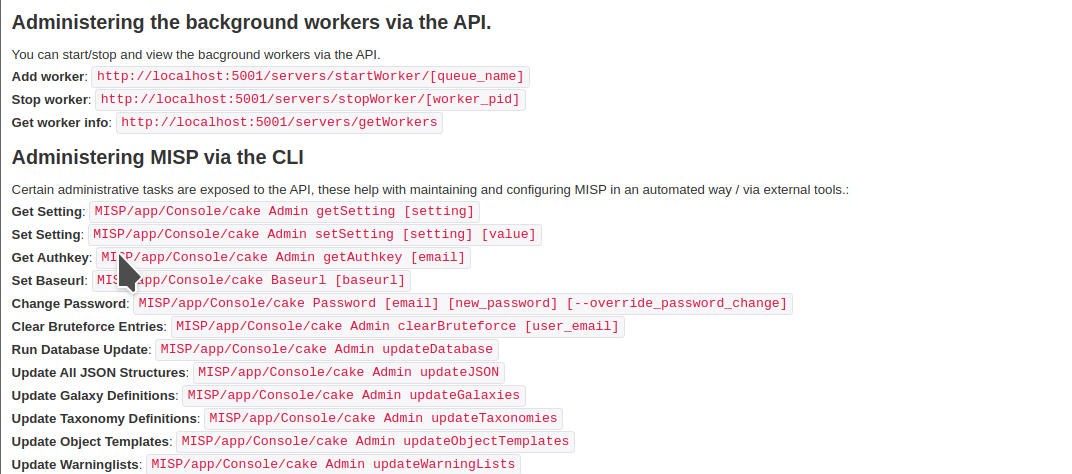
\includegraphics[scale=0.4]{cli.png}
  \end{center}
\end{frame}

\begin{frame}
\frametitle{Usage}
    \texttt{/var/www/MISP/app/Console/cake [Shell] [Command] [parameters]}
    \begin{itemize}
        \item Example:
        \begin{itemize}
            \item \texttt{/var/www/MISP/app/Console/cake Password "andras.iklody@gmail.com" "Nutella"}
            \item Change password to "Nutella" for my user
            \item Some shells are single use and don't need a command parameter
        \end{itemize}
        \item Also used by the background processing
        \item Automation is meant to be used via cron jobs
    \end{itemize}
\end{frame}

\begin{frame}
\frametitle{Automation via crontab}
    \begin{itemize}
        \item Edit crontab of www-data user
        \item \texttt{crontab -u www-data -e}
        \item \texttt{0 3,9,15,21 * * * /var/www/MISP/app/Console/cake Server pull 1 30 full}
        \item Pull server ID \#30 as user \#1 every 6 hours
        \item \texttt{@hourly /var/www/MISP/app/Console/cake Server cacheFeed 1 csv full}
        \item Cache all csv feeds as user \#1 every hour
    \end{itemize}
\end{frame}



